\documentclass{udthesis}

\usepackage[english]{babel}
%\usepackage{float}
%\usepackage[hidelinks]{hyperref}
\usepackage{graphicx}
\usepackage{bookmark}

\makeatletter
\providecommand{\toclevel@prefacesection}{0}
\makeatother

\usepackage[usenames,dvipsnames]{xcolor}
\usepackage{tcolorbox}
\usepackage{tabularx}
\usepackage{array}
\usepackage{colortbl}
\tcbuselibrary{skins}

\pdfoptionpdfminorversion=7

\definecolor{myblue}{RGB}{72,107,123}
\definecolor{myblue2}{RGB}{184,206,216}
\definecolor{darkgreen}{RGB}{0,151,33}

\newcolumntype{Y}{>{\centering\arraybackslash}X}
\tcbset{borderline={0.5mm}{0.0mm}{myblue},sharp corners,width=1.0\textwidth,enhanced,boxrule=0.5pt,fonttitle=\normalsize,
colback=gray!01!white,colframe=myblue,colbacktitle=myblue2,
coltitle=black,center title,shrink tight}

\newcommand{\unt}[2]{\mbox{#1\,#2}}

%\usepackage{draftwatermark}
%\SetWatermarkScale{8}
%\SetWatermarkLightness{0.96}

\begin{document}
    %FIXME: FIX NUMBERING of pages to romane numerals, Get required pages (see Josh's thesis), add Acknowledgment.
    \title[TBD]{TBD}
    \author{Aaron Myles Landwehr}
    \type{dissertation}
    \degree{Doctor of Philosophy}
    \majorfieldtrue\majorfield{Electrical \& Computer Engineering}
    \degreedate{Spring 2020}
    \keywords{tbd}
    \subject{Subject}

    \maketitlepage

    \begin{approvalpage}
    \chair{Kenneth E. Barner, Ph.D.}{Chair of the Department of Electrical and Computer Engineering}
    \dean{Levi T. Thompson, Ph.D.}{Dean of the College of Engineering}
    \provost{Douglas J. Doren, Ph.D.}{Interim Vice Provost for Graduate \& Professional Education and Dean of the Graduate College\par}
    \end{approvalpage}

    \begin{signedpage} % Up to 4 signatures
        \profmember{Fouad E. Kiamilev, Ph.D.}
        \member{Chase J. Cotton, Ph.D.}
        \member{Xiaoming Li, Ph.D.}
        \member{St\'ephane Zuckerman, Ph.D.}
    \end{signedpage}

    \begin{front} % Starts front material (Roman style page numbers)
        \prefacesection{Acknowledgments}
            Firstly, I would like to thank my mother for pushing me to get a college education over all of the years of my life. Secondly, I would like to thank Moon for being a loner cat and letting me spend long nights on campus finishing my thesis. Thirdly, I would like to thank all of the current and former members of my research group, CAPSL, for helping educate and train me, as well as, for providing input toward the pursuit of my research. Fourthly, I would like to thank Jose Monsalve for being a good friend and pushing me to be a happier person in a time when I needed the support. Fifthly, I would like to thank Laura Rozo Duque for helping provide me with a path to exploring myself as a unique individual human being. Finally, I would like to thank Muffin for his chews straight to the heart. 

        %\tablespagefalse
        \maketocloflot
        \prefacesectiontoc{Abstract}
            %FIXME: get rid of we
Traditional display protocols have limitations in terms of fixed frame rates, high bandwidth requirements, and precise control over the display of frames. We propose a novel scalable packetized display protocol architecture incorporating dynamic frame rates, high-speed capabilities, and dynamic synchronization to bridge performance gaps. We further provide a modular FPGA implementation of the architecture for use on array emitters.

    \end{front}

    \pagenumbering{arabic}

    \chapter{Introduction}
        \label{chap:introduction}

Infrared Scene Projection Systems (IRSPs) are emerging as a novel technology for the testing and development of IR based sensor technology and real-time IR simulations. They provide a compelling alternative to the older entrenched technology of resistor-array based IR scene projector systems\cite{pritchard1998design,williams2005history} due to various improvements over the competing technology. These improvements include but are not limited to better maximum apparent temperature (above 1400 Kelvin), better dynamic range, higher pixel density (24 micrometers and lower), substantially faster emission in the target spectrums with optical rise-times in the nanoseconds. Additionally, they are relatively difficult to damage thermally and have the potential to provide emission in multiple spectrums through what are termed "multi-color" pixels. The latter, refers simply to the fact that IRLEDs can be designed for multi-spectral emission.

Current fixed framerate display technology, such as, DVI\cite{DDWG1999}, HDMI\cite{HDMIForum2018}, and DisplayPort\cite{BhowmikEtAl2012} are commonly utilized technologies within IRSP and resistor array systems. They provide a standardized method to transmit digital scene data which is then translated into analog signaling for display on IR arrays. However, within IRLED systems which are inherently fast and primarily limited by electronics, these technologies have become limiting for high-speed IR display\cite{EjzakEtAl2016,LaVeignePrewarski2013}.

These display technologies, designed for relatively low-speeds (generally 60Hz until recently) incorporate a number of design decisions that limit the ability to utilize them effectively with IR emitter technology. Firstly, these technologies require custom designed synchronization solutions and hardware when utilized with multiple sources in order to ensure correct synchronization because they are not designed to handle synchronization across multiple sources. For example, display walls may utilize Quadro Sync Cards\cite{NVIDIAQuadroSync} to provide synchronization across multiple monitors; however, this only provides a coarse-grain synchronization within one frame of latency between the displays. Secondly, the fixed frame rate nature of technology imposes a static requirement on frame rate across all displayed frames increasing bandwidth requirements by requiring the same amount of data be sent for all frames regardless of what data changes. This necessarily means that maximum frame rate operation is limited by the resolution size of imagery due to bandwidth limitations across physical links. This relationship between frame size and bandwidth is discussed in more detail in Chapter \ref{chap:problem_formulation}.

In this dissertation, we propose an alternative to traditional display technology, a packetized display protocol (PDP) architecture capable of providing a synergy with the the benefits of IRSP technology in order to bridge the performance gap of ever the increasing speed requirements of high speed projector systems. Sensor technology can operate in ranges of above one kilohertz which represents an order of magnitude difference to the current target speeds of fixed-rate display technology. This PDP architecture eschews with many of the assumptions found within traditional display technology in order to provide scalability, reduce bandwidth requirements, increase performance, ease synchronization burden; as well as; provide a desirable set of features, such as, dynamic sub-window frame rates not found within current fixed-rate technology. This architecture demonstrates that with the proper set of control and features, high-speed operation can be achieved even with limited physical bandwidth.
%FIXME: do kilohertz sensors exist?

Our protocol architecture draws inspiration from the video processing field, where encoding schemes for video streaming represent a body of research that attempts to tackle a similar but more limited challenge\cite{BakarEtAl2017}. Some of these encoding schemes attempt to provide a variable frame rate for segments of the incoming stream through differencing algorithms, but also rely on compression\cite{CastilloEtAl2012} which reduces quality and introduce artifacts. These technologies will be discussed more thoroughly in Chapter \ref{chap:related_work}. In our case, we require lossless quality; and thus, cannot utilize these for our purposes. Instead, we seek to craft a lossless solution for the IRLED projector field that incorporates similar variable frame rate features in order to reduce bandwidth consumption, as well as, allow bandwidth to used more intelligently. More specifically, we envision apportioning avaliable bandwidth to regions of a scene that necessarily need to update frequently. In IR scenes, this generally includes regions that transition from dark to light or light to dark quickly, and higher temperature regions. Regions which do not change temperature quickly, generally do not need updated as often due to charged LEDs holding capacitance for milliseconds at a time\footnote{The general time of discharge depends on the design of the LEDs and amount of charge currently held within. However, we have measured \textgreater1 millisecond in test setups.}.
%FIXME: How long to LEDs actually hold capacitance, and is there a citation I can use?

The contributions of this dissertation are as follows: firstly, we provide the architecture of a physical layer agnostic packetized display protocol with the following features (1) intelligent dynamic per-frame bandwidth utilization, (2) fine-grained control over frame transmission and synchronization, (3) dynamically changing intra-frame rates, and (4) a realized implementation of the protocol for use on array emitter technology. Within we discuss relevant details of the initial design, methodology, and implementation of the said protocol. Secondly, we provide a sufficiently abstract machine model to indicate a path to utilize the protocol within current and future systems. Thirdly, we demonstrate the use of the protocol within real IRSP systems, as well as, provide the current results and a comparison with fixed-rate technology. Fourthly, we discuss various use-cases for the technology to provide the reader with a more complete understanding of where this technology could be utilized in future systems.

This dissertation is divided into the following sections: background; which discusses the various aspects of current IRSP systems that are relevant to understanding PDP, problem formulation; which examines the problem of high speed projection in detail, packetized display protocol; which discusses the design methodology and the rationale for PDP, machine model; which discusses the overall abstract PDP architecture, use cases; which examines utilizing PDP within real systems, implementation; which discusses an implementation of the protocol on an FPGA system and provides experimental results, related work; which discusses relevant work within the field of high-speed display systems techology, and the conclusion; which discusses the future of PDP and potential avenues of further research.

    \chapter{Background}
        \label{chap:background}

 This chapter discusses relevant background information toward the goal of implementing a packetized display protocol (PDP) architecture for Infrared Scene Projector systems (IRSPs). First, it gives an overview of what constitutes an IRSP system. Following this, it provides a general discussion of how common display protocols work to send pixel data to a display system (e.g. a television). Finally, it discusses how these protocols are utilized within an IRLED project system including discussion of example scenarios.

\section{IRLED Projector Systems}

\begin{figure}
    \centering
    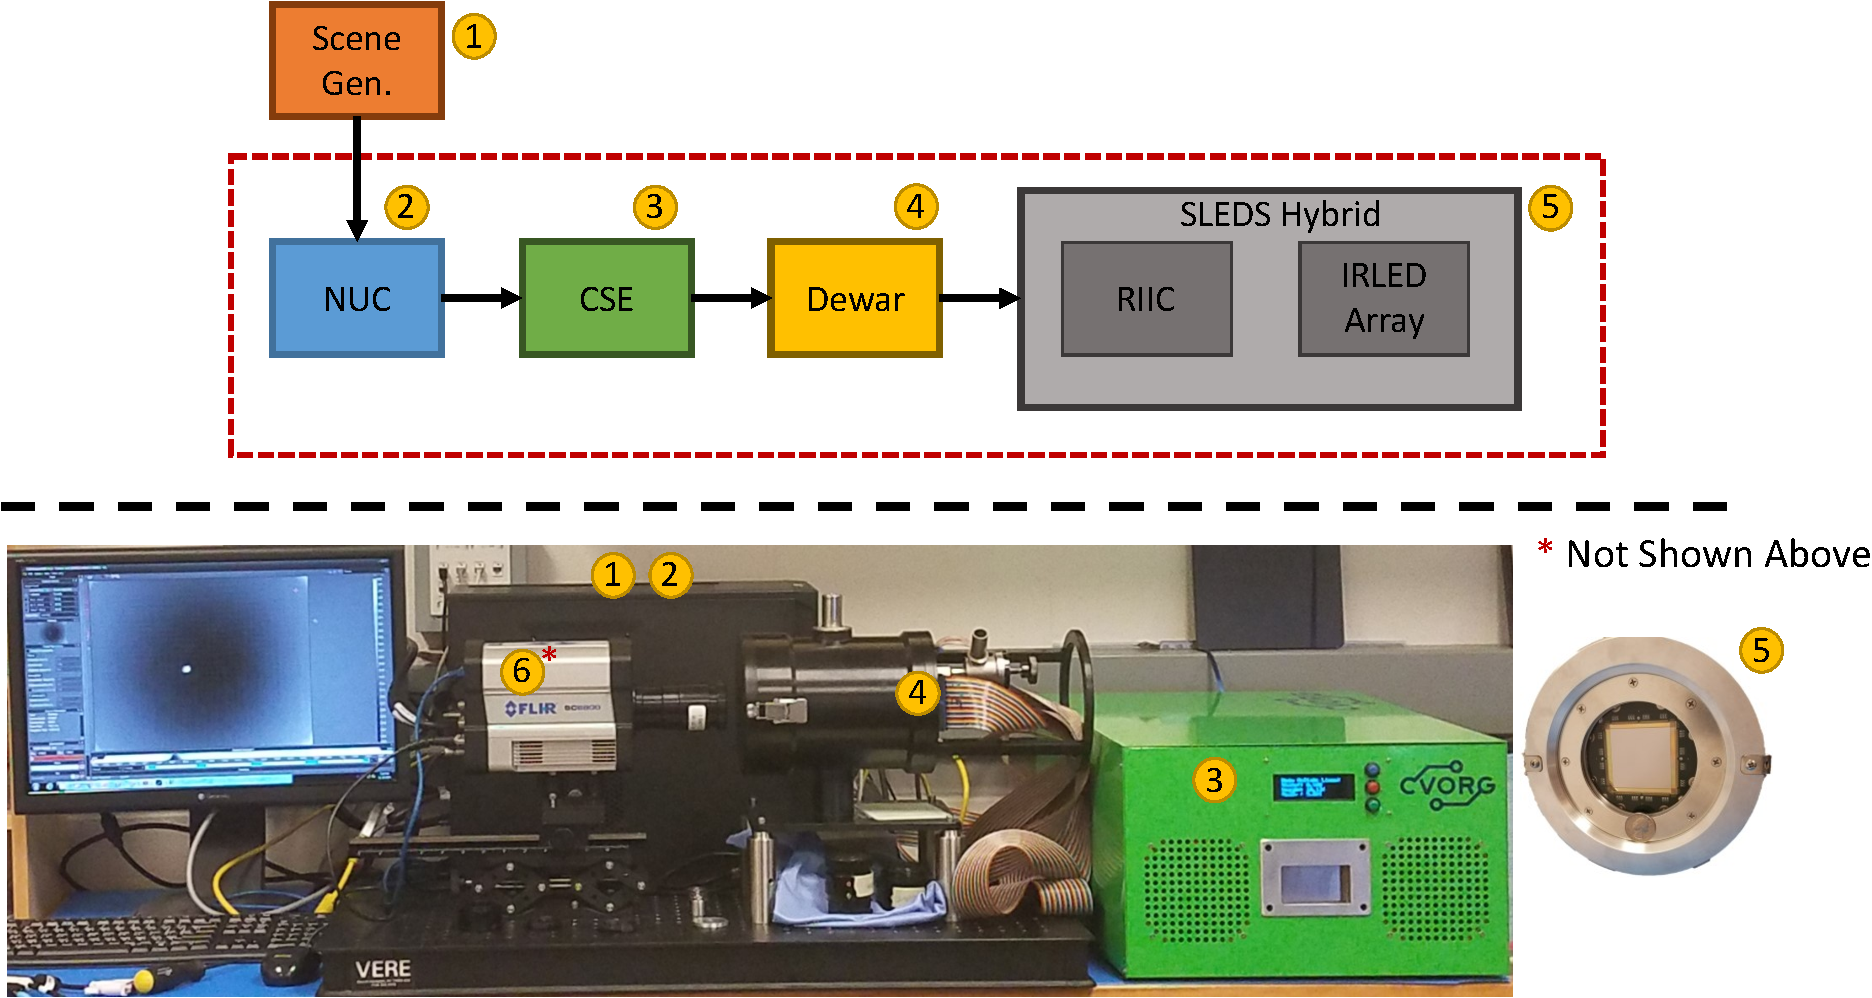
\includegraphics[width=1.0\textwidth]{fig/sleds_system.pdf}
    \caption{IRLED Scene Projector System}
    \label{fig:sleds_system}
\end{figure}

IRLED based IRSPs are made up light emitting diodes (LEDs) that emit light in the IR spectrum\cite{biard1966semiconductor}. Since their inception they have been utilized in various fields such as medical\cite{MonteiroEtAl2011,MEEKS1998433,Sadick2009,takhtfooladi2015effects,yamanishi1995respiration} sensing; tracking; and localization\cite{PlotogVladescu2015,Kimon2001,SCHOLZ20151233,WalshDaemsSteckel2015,zeylikovich2003mid}, and communication\cite{CossuEtAl2014,escobosa2004ir,GeorgopoulosKormakopoulos1986,sohn2007localization,JangEtAl2012}. IRLED projectors are an emerging technology with various applications within the IR sensor testing community. A complete IRLED based IRSP system consist of various technologies and processes as shown in Figure~\ref{fig:sleds_system}. One denotes the scene generation and non-uniformity correction (NUC) process. This is where pixel data representing IR scenes is fed to a system for display. The NUC process is for correcting for physical and thermal non-uniformity in an IRLED array\cite{BarakhshanEtAl2018}. Two denotes the close support electronics which are responsible for converting a digital representation of a scene into analog signaling that goes directly to an array. Three indicates the dewar or vaccum chamber which houses an IRLED array and is utilized to keep it below ambient temperatures or at cryogenic temperature ranges. Four indicates an IRLED hybrid which consist of a Read-in Integrated Circuit (RIIC) used to address an IRLED array and the array itself. Analog signals coming from the CSE go into the dewar, and then are mapped using the RIIC, which results in specific IRLEDs within an array being driven. Five indicates an IR recording apparatus of some sort utilized to record IR data from an array. Synchronization between source generation, display, and recording is maintained via synchronization signaling. Often Camera Link serial communication\cite{CameraLink2000,zhu2008design} is used.


Figure~\ref{fig:sleds_timeline} shows the development timeline for IRLED Projector technology. In 2008, the world's first IRLED array called the Superlattice Light Emitting Diodes (SLEDs) array was completed in 2008\cite{ahmed1}.

\begin{figure}
    \centering
    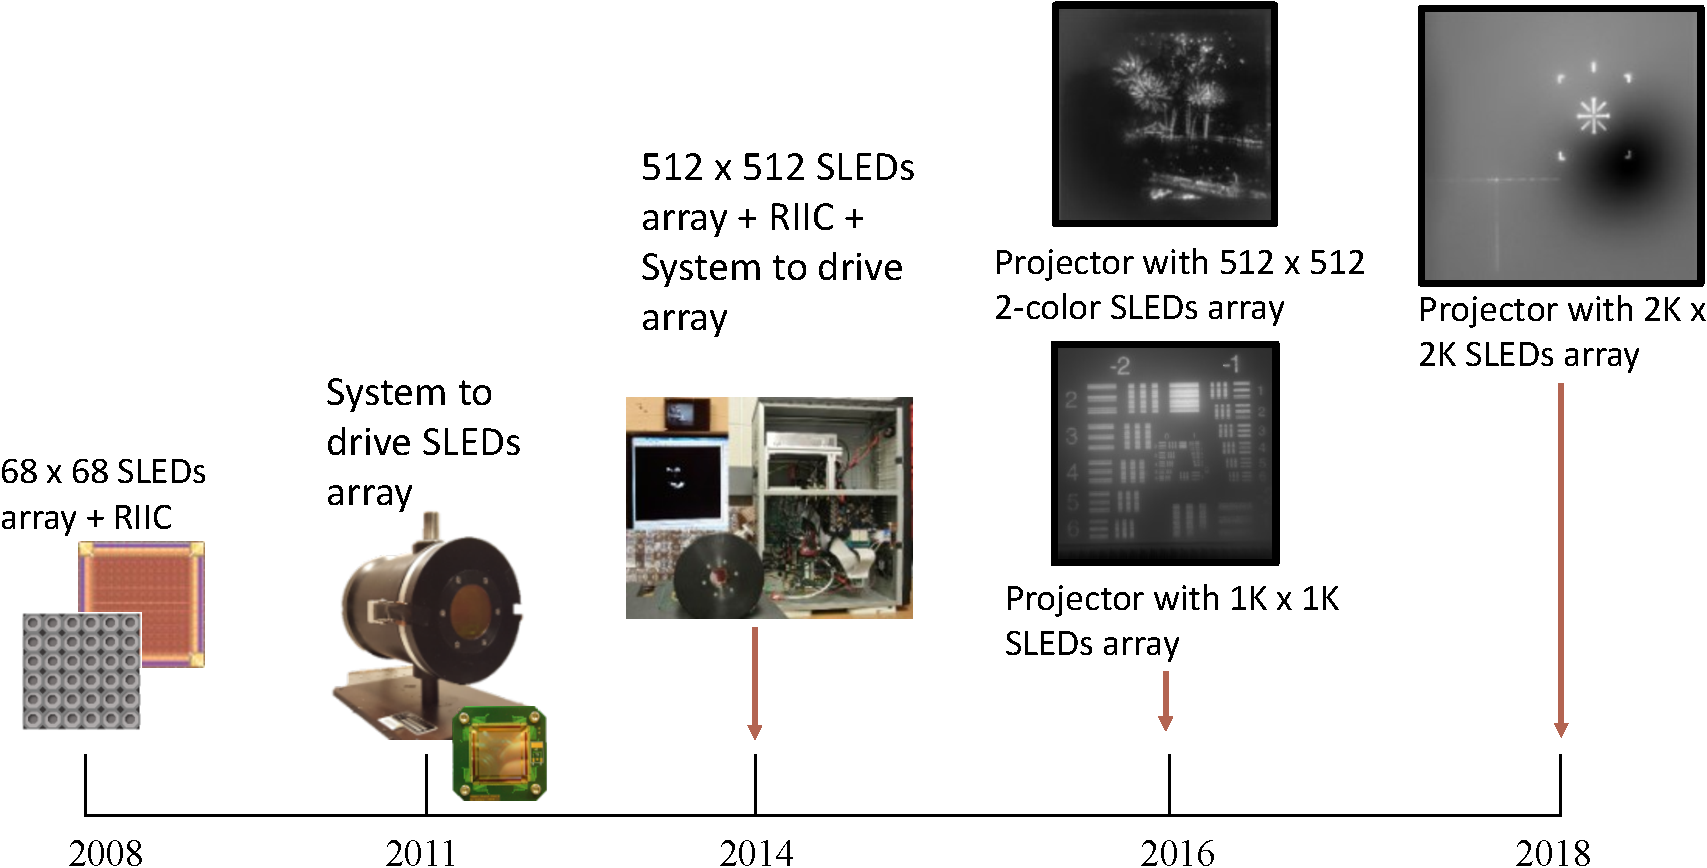
\includegraphics[trim=1.5in 0.5in 1.5in 1.5in,width=1.0\textwidth]{fig/sleds_timeline.pdf}
    \caption{IRLED Projector Technology Development Timeline Overview}
    \label{fig:sleds_timeline}
\end{figure}

This device was a hybridized combination of an 68 by 68 IRLED wafer bonded to a RIIC wafer providing the electronics to drive the array. Initial testing was done by hand prior the design and implementation of the overall drive system was completed in 2011. Following this, an increased IRLED wafer of 512x512 size was fabricated in 2014. These efforts culminated in the first two IRLED projector systems in 2016. The first, a 512 by 512 sized array included support for driving the LEDs at two separate wavelength bands (denoted as 2-colors in Figure~\ref{fig:sleds_timeline})\cite{EjzakEtAl2016, RickerEtAl2017}. The second, a 1024 by 1024 sized array doubled the total number of pixels supported. Additionally, these systems demonstrated the beginnings of a modular IR Scene Projection (IRSP) platform\cite{BrowningEtAl2019}. A further increase in size and efficiency occurred in 2018 with the world's first 2048 by 2048 pixel array.

\begin{figure}
    \centering
    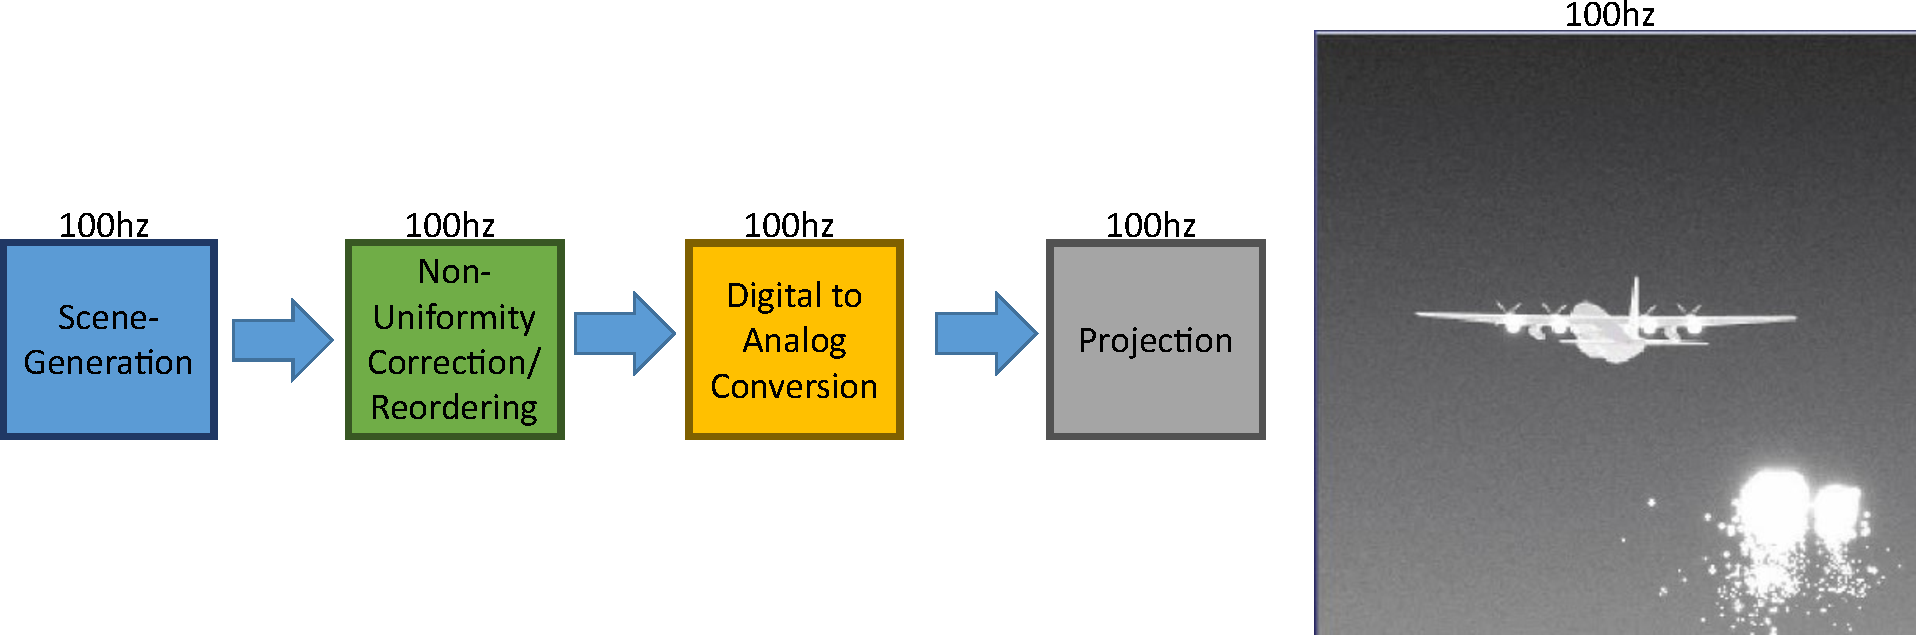
\includegraphics[trim=1.5in 0.5in 1.5in 1.5in,width=1.0\textwidth]{fig/typical_projection_system.pdf}
    \caption{Typical IRLED Projection Process}
    \label{fig:typical_projection}
\end{figure}

%FIXME: add discussion about the speeds

%FIXME: add discussion about uses

%FIXME: add discussion about system layout


\section{Classical Display Protocols}
    \label{sec:classical_display_protocols}

    Classical display protocols such as (DVI\cite{DDWG1999}, HDMI\cite{HDMIForum2018}, and DisplayPort\cite{VESA2016} are commonly used for driving consumer electronic devices. These generally provide a standardized feature-set that is rooted in classical analog video specifications (e.g. VGA, Composite)\cite{NIAnalog} that utilize scan lines\cite{Neal1998}. Scan lines are used to provide video timing information in order to synchronize a display to a given refresh-rate. Each scan line consist of an active video region followed by a horizontal blanking period. After all active video scan lines are displayed, a vertical synchronization region is used to indicate the end of a frame.

    \begin{figure}
        \centering
        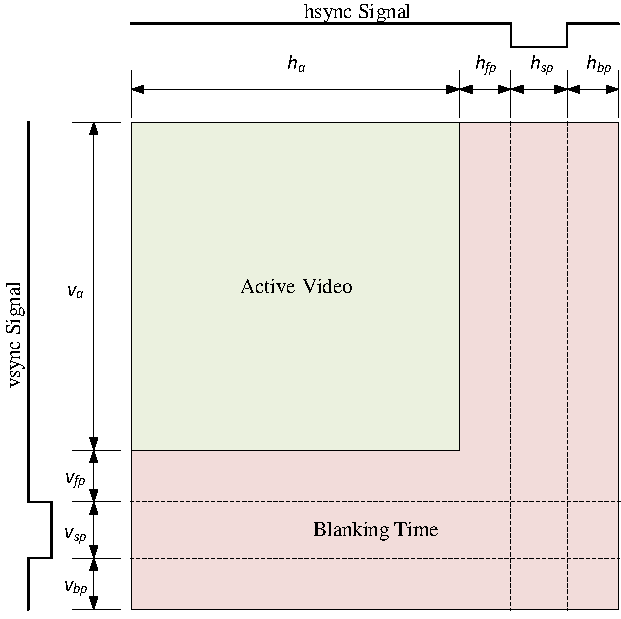
\includegraphics[width=1.0\textwidth]{fig/display_timing_overview.pdf}
        \caption{Display Protocol Timing Overview}
        \label{fig:display_protocol_timing_overview}
    \end{figure}

    \begin{figure}
        \centering
        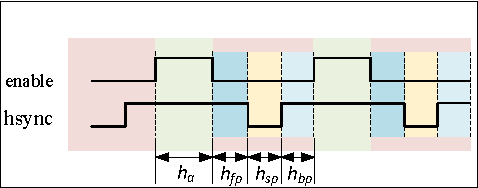
\includegraphics[width=1.0\textwidth]{fig/display_timing_line_cross.pdf}
        \caption{Display Protocol Horizontal Signal Cross Section Timing}
        \label{fig:display_protocol_line_cross}
    \end{figure}

    %FIXME add crosssectional blowout chart

    An overview of this is shown in Figure~\ref{fig:display_protocol_timing_overview}. The region shown in green is the pixel data for the active video region of the display. It is of size $H_a\times V_a$ which represents the number of pixels to display, for example, 1920 by 1080 for a HDTV high-definition video mode\cite{MythTVWebsite}. The blanking time regions denote pixel data that is sent but not displayed\footnote{Typically data lines are held low during this period, but somtimes it is used for out-of-band communication to send other information such as audio encoding.}. A scan line consist of pixels made up of $h_a$, the horizontal active size; $h_{fp}$, the horizontal front porch before the pulse signal; $h_{sp}$, the horizontal sync pulse; and $h_{bp}$, the horizontal back porch after the sync pulse. The vertical blanking period makes up multiple scanlines and consist of $v_{fp}$, the vertical front porch before the vsync pulse; $v_{sp}$, the vertical sync pulse; $v_{bp}$, the vertical back porch after the vertical sync pulse. Sync pulses are generally active low, meaning that during active display a sync signal is high as shown in the diagram.

    Figure~\ref{fig:display_protocol_line_cross} shows a closeup view of signal lines during the active region of display for two scan lines. A data enable signal denoted by $enable$ is high during the active region shown in green. Following this, it goes low for a period of time denoted by $h_{fp}+h_{sp}+h_{bp}$. The horizontal sync signal goes low only in the region shown in yellow between the front porch and back porches. This process repeats for all scan lines. Once the last active region pixel is drawn, the enable signal will stop going high during the vertical synchronization period.

    %FIXME: Fix discussion of DP not using fucking backwards compatibility shitty hdmi fucking mode
    %FIXME: Talk about CC in the vertical blanking

    \begin{figure}
        \centering
        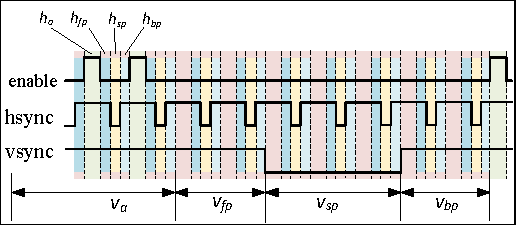
\includegraphics[width=1.0\textwidth]{fig/display_timing_full_cross.pdf}
        \caption{Display Protocol Full Signal Cross Section Timing}
        \label{fig:display_protocol_full_cross}
    \end{figure}

    Figure~\ref{fig:display_protocol_full_cross} shows a closeup view of signal lines during the transition into the vertical synchronization period. The region donated by $V_a$ indicates the end of the video active region of the display which occurs toward the end of a frame. After the active video region, all data has been drawn to a display. The region denoted by $v_{fp}+v_{sp}+v_{bp}$ is the vertical blanking or vsync period during which no active video data is sent; therefore, data enable denoted by $enable$ is always low during this period. Before the vertical sync pulse period denoted by $v_{sp}$ occurs, a vertical front porch period denoted by $v_{fp}$ occurs. After the vertical sync pulse, a vertical back porch region $v_{bp}$ occurs. Following this the beginning of the next frame occurs as denoted by $v_{a+1}$.
    \begin{figure}
        \centering
        { \Large
            $l_h=h_a+h_{fp}+h_{sp}+h_{bp}$ \vspace{8px} \\
            $l_v=v_a+v_{fp}+v_{sp}+v_{bp}$ \vspace{8px} \\
            $f_f={f_p \over {l_h \cdot l_v}}$ \\
            $p_t={1 \over f_p}$ \vspace{8px} \\
            $f_t={1 \over f_f}$ \vspace{8px}
        }
        \caption{Total Refresh Rate}
        \label{fig:modeline_refresh_rate}
    \end{figure}

    Figure~\ref{fig:modeline_refresh_rate} shows the relationship between between the different regions of a display and the frequency or refresh rate. $l_h$ denotes the scan line size of a display, or total horizontal width, which is made up of the horizontal active and horizontal porch region pixels of a display. $l_v$ denotes the total vertical width of a display, which is made up the vertical active and vertical porch region pixels of a display. Each pixel is sent at a rate denoted by $f_p$, the pixel frequency (also called the pixel clock). $f_f$ denotes the frame frequency or framerate of a display. This is simply the pixel frequency over the total number of pixels (video active and porches) of a display. $p_t$ denotes the time period a single pixel takes to send. $f_t$ denotes the time period for an entire frame.

    %FIXME: example modeline
    To illustrate, let us look at the display modeline generated using the VESA Coordinated Video Timing (CVT) standard shown in Figure~\ref{fig:modeline_example}. This modeline operates a total frame frequency of approximately \mbox{30 Hz}. The pixel clock 79.75, denoted in red, is specified in megahertz. The horizontal pixels, denoted in blue; are the end of horizontal active, the end of horizontal front porch, the end of horizontal sync pulse, and the end of horizontal back porch respectively. The vertical pixels (measured in lines), denoted in green; are the end of vertical active, the end of vertical front porch, the end of vertical sync pulse, and the end of horizontal back porch respectively. The sync pulse polarities, denoted in yellow; indicate whether a given sync pulse is active low or active high. A minus symbol indicates active low and a plus symbol indicates active high. If these numbers are placed into into the formulas shown in Figure~\ref{fig:modeline_refresh_rate} the results shown in Figure~\ref{fig:modeline_refresh_rate_plug} are yielded. The astute reader will note that $l_h$ and $l_v$ are the same as the total pixel size for the given modeline. The pixel period is $\sim12.53ns$, meaning that each pixel is drawn for the given amount of time. The frame period is $\sim33.33ms$, meaning that each frame is drawn for that given amount of time.

    \begin{figure}
        \centering
        { \normalsize
        \textbf{``1920x1080\_30.00"} {\color{red}79.75}  {\color{blue} 1920 1976 2168 2416}  {\color{darkgreen}1080 1083 1088 1102} {\color{olive}-hsync +vsync}
        %\vspace{-8px}
        }
        \caption{VESA CVT Generated Modeline}
        \label{fig:modeline_example}
    \end{figure}

    %FIXME: finish this chart
    \begin{figure}
        \centering
        { \Large
            $h_a=1920; h_{fp}=1976-h_a; h_{sp}=2168-h_{fp}; h_{bp}=2416-h_{sp};$ \\
            $v_a=1080; v_{fp}=1083-v_a; v_{sp}=1088-v_{fp}; v_{bp}=1102-v_{sp};$ \\
            $l_h=2416=1920+56+192+248$ \vspace{8px} \\
            $l_v=1102=1080+3+5+14$ \vspace{8px} \\
            $f_p=79.75e6$ \vspace{8px} \\
            $f_f=30.0={f_p \over {l_s \cdot l_c}}$ \\
            $p_t=12.53ns={1 \over f_p}$ \vspace{8px} \\
            $f_t=33.33ms={1 \over f_f}$ \vspace{8px}
        }
        \caption{Computed Refresh Rate for a 30hz CVT Modeline}
        \label{fig:modeline_refresh_rate_plug}
    \end{figure}

    Section~\ref{sec:displays_within_proj_system}, discusses how these protocols are utilized within an IRLED projector system, briefly highlight the limitations, and . %FIXME: finish this paragraph

\section{Display Protocols within an IRLED Project System}
    \label{sec:displays_within_proj_system}
    Projector systems utilize

    \chapter{Problem Formulation}
        \label{chap:problem_formulation}

 In this chapter, we will discuss in detail the limitations with current display protocol technology that were alluded to in Chapter \ref{chap:introduction}. From there, we will focus on how these limitations affect adversely IRLED projector technology. Finally, we will provide a problem solution.

\section{Problem Statement}

\subsection{Display Protocol Limitations}

\subsection{High-speed IRLED Projector systems}

\section{Problem Solution}

As discussed briefly in the section \ref{chap:introduction}, our PDP architecture eschews with assumptions found in traditional display technology in order to provide a rich set of desirable features. In this section, we will discuss the assumptions of traditional display technology and how PDP differs, in order to provide the reader a rationale, as well as, the benefits to our proposed alternative.

Current display technology, such as HDMI, assumes a fixed frame rate display which places a hard limit on frame timing and synchronization. In detail, the underlying display protocols operate in a best-effort fashion where a buffer swap transmitting a frame of data occurs at static predetermined interval. If a new frame is unavailable to be transmitted at each interval due to any delay, such as processing delay, the previous frame will be retransmitted. This necessarily makes correct synchronization challenging because modern computation systems do not generally provide real-time guarantees for a number of reasons, such as, variability in work needed for frame generation, CPU scheduling, and I/O delays. Generally, while these challenges can be addressed to some degree, they require custom hardware solutions on top of existing display protocols because end-to-end system synchronization is out of the scope of typical display standards which are designed to push relatively low frame rates over single hardware links. Secondly, because of the static nature of of the transmission interval (e.g. 100hz), the frame rate cannot be dynamically controlled or changed after initialization. Instead, these protocols have static bandwidth requirements for a given resolution and frame rate of the form found in figure \ref{fig:bandwidth}. This disallows for fine-grained control over the frame rate in cases where a user might wish to dynamically change it to match the processing rate. In high speed display scenarios, this introduces the problem of unavoidable frame drops. This issue becomes further compounded by the fact that traditional display protocols utilize proprietary drivers and hardware such that frame-drops become effectively silent. An effort to address this problem necessarily requires complete control over the entire end-to-end system meaning an effective and correct solution requires customized hardware and software that deviates from standard display protocol behavior. Any solution that falls short of these requirements would necessarily fail to completely address the issue. In short, to truly address this issue within traditional display protocols would require essentially creating device specific new protocol tied to particular custom hardware. Finally, display protocols disallow the transmission of sub-frames of data. A frame is necessarily transmitted in whole when the transmission interval reached. Just as with the previous problem, to alleviate this would necessarily require control over driver and hardware behavior in an end-to-end system.

\begin{figure}
    \centering
    \large
    %\begin{small}
    %$$bandwidth = resolution \times bits \times fps$$
    %$bandwidth$ : \quad bandwidth requirements in bits per second. \\
    %$resolution$ : \quad number of pixels including porches. \\
    %$bits$ : \quad \quad \quad \ \ \ bits per pixel. \\
    %$fps$ : \quad \quad \quad \ \ \ frames per second.
    \begin{tabular}{| r l |}
        \hline
        $$bandwidth$$ & = resolution $\times$ bits $\times$ fps \\ \hline
        $bandwidth$ & : bandwidth requirements in bits per second. \\
        $resolution$ & : number of pixels including porches. \\
        $bits$ & : bits per pixel. \\
        $fps$ & : frames per second. \\
        \hline
    \end{tabular}
    \caption{Bandwidth requirements of a traditional display protocol}
    \label{fig:bandwidth}
    %\end{small}
\end{figure}

Our proposed architecture, on the other hand, is designed to utilize a dynamic source driven refresh rate through the coordination of both source (scene generator) and sink (display). In this architecture, frames are segmented into pieces or sub-frames and sent to the display based upon how often these segments need to update. An example of this is shown in figure \ref{fig:variable_display} where different regions of the display operate at different frame rates. By utilizing dynamic frame rate control at sub-frame resolutions, substantial bandwidth reductions can occur. This will be discussed in further detail in subsequent sections.

The underlying PDP protocol itself is designed to allow for fine-grained control over when and what data is transmitted, incorporate mechanisms to synchronize and eliminate frame-jitter. Furthermore, the protocol architecture is abstracted in such a way that the physical interconnect layers are transparent in order to enable it to be capable of operating over a wide-spectrum of hardware, as well as, to future proof the protocol for use in future hardware. This enables a risk-reduction for the utilization of the protocol in that a hardware system implementing this protocol could switch or upgrade physical components and still utilize the same protocol within the software stack given an appropriately compatible physical layer. To facilitate this, we have chosen a packetized protocol structure capable of transmitting pixel data in a generalized way. In the subsequent section we will discuss the architecture of our protocol.

    \chapter{Packetized Display Protocol}
        \label{chap:pdp_protocol}

In this Chapter, we discuss the underlying communication details of our packetized display protocol (PDP) architecture. First, we give an overview of the protocol design methodology. Followed by a discussion of the generalized packet format. Finally, we discuss individual packet types. The central purpose of this chapter is to provide the reader with an understanding of the reasoning behind design decisions, as well as, to provide a detailed specification of the protocol.

\section{Design Methodology}

    The design methodology for the PDP protocol began with a number of critical design goals. The first goal was to design a scalable display system that was distributable and hardware agnostic. The second design goal was to provide a protocol that was relatively simple to implement without unnecessary complexity to ease the encoding and decoding process. Additionally, simplifying these processes eases potential hardware implementation mistakes, as well as, inefficiencies that could lead to reduced performance. The third goal was to provide dynamic intra-frame variable refresh rate (VRR) to enable better bandwidth utilization as shown in figure \ref{FIXME}. In particular, to allow for regions of a display to be intelligently updated at different rates depending differences in input data. The fourth goal was to provide a path to utilize classical display protocol streams such as HDMI with PDP without introducing overhead. This is to allow for interoperability where necessary when utilizing classical display sources.

    \subsection{Comparison to Classical Display Protocols}

        In order to better understand how to design PDP, we investigated the constraints of classical display protocols in order to discern which features within these conflicted with our design goals. In addition, we wanted to investigate whether these could provide a direction for where to go with PDP. Many of the older and newer versions of these protocols (DVI\cite{DDWG1999}, HDMI\cite{HDMIForum2018}, DisplayPort\cite{VESA2016}, etc.) provide similar feature-sets to end-users with the major focus being on increasing refresh-rates and resolutions with each new specification. However, as noted in Section \ref{sec:classical_display_protocols}, their basis is rooted in the classical analog video specifications which utilize scan lines\cite{Neal1998}. This means, that signal timing utilizes vertical and horizontal blanking periods that consist of a front-porch, sync pulse, and back-porch; in addition to, the active video data to be displayed.

        \begin{table}
            \centering
            \large
            \begin{tcolorbox}[tabularx={Y|Y|Y|Y|Y},title=\textbf{Modeline Overhead},boxrule=0.5pt]
            \textbf{Resolution} & \textbf{Refresh-Rate (Hz)} & \textbf{Visible Pixels} & \textbf{Total Pixels} & \textbf{Overhead} \\ \hline
                \textbf{1920x1080} & \textbf{60}   & 2073600 & 2475000 & 16.2\% \\ \hline
                \textbf{1600x1200} & \textbf{60}   & 1920000 & 2700000 & 28.9\% \\ \hline
                \textbf{1280x1024} & \textbf{60}   & 1310720 & 1799408 & 27.2\% \\ \hline
                \textbf{1280x960}  & \textbf{60}   & 1228800 & 1800000 & 31.7\% \\ \hline
                \textbf{1280x800}  & \textbf{60}   & 1024000 & 1391040 & 26.4\% \\ \hline
                \textbf{1024x768}  & \textbf{60}   & 786432  & 1083264 & 27.4\% \\ \hline
                \textbf{500x500}   & \textbf{500}  & 250000  & 296100  & 15.6\% \\ \hline
                \textbf{500x500}   & \textbf{400}  & 250000  & 296100  & 15.6\% \\ \hline
                \textbf{500x500}   & \textbf{300}  & 250000  & 357500  & 30.1\% \\ \hline
                \textbf{500x500}   & \textbf{100}  & 250000  & 357500  & 30.1\% \\ \hline
                \textbf{500x500}   & \textbf{60}   & 250000  & 357500  & 30.1\% \\ \hline
                \textbf{500x500}   & \textbf{50}   & 250000  & 364000  & 31.3\% \\ \hline
                \textbf{500x500}   & \textbf{30}   & 250000  & 520000  & 51.9\% \\ \hline
                \textbf{500x500}   & \textbf{30}   & 250000  & 520000  & 51.9\% \\ \hline
                \textbf{500x256}   & \textbf{1000} & 131072  & 149460  & 12.3\% \\ \hline
                \textbf{500x256}   & \textbf{500}  & 131072  & 256000  & 48.8\% \\ \hline
                \textbf{500x256}   & \textbf{200}  & 131072  & 320000  & 51.9\% \\ \hline
                \textbf{500x256}   & \textbf{100}  & 131072  & 320000  & 59.0\% \\ \hline
                \textbf{500x256}   & \textbf{60}   & 131072  & 320000  & 59.0\% \\ \hline
            \end{tcolorbox}
            \caption[Modeline Overhead]{Modeline overhead for various resolutions and refresh rates\cite{MythTVWebsite}. Computed using active pixel area over total pixel area. 500x500 and 512x256 are typical modeline resolutions used on IRLED arrays.}
            \label{tbl:modeline_overhead}
        \end{table}

        For analog display devices, these signals enabled operators to manually adjust horizontal and vertical hold times relative to the sync pulses in order to correct for the imprecise timing of early display hardware; but provide little benefit on modern hardware. Instead, they represent an anachronism that impedes the goal of maximizing bandwidth utilization to a display by requiring the transmission of unnecessary data over a digital protocol. For example, a commonly utilized 1920 by 1080 pixel mode operating at 60 hertz\cite{MythTVWebsite} on a modern display has a 16 percent blanking period overhead due to the specification of vertical and horizontal sync periods. Other examples can be seen in Table \ref{tbl:modeline_overhead}.

        These protocols also internally utilize a mode based display of data that requires the specification of the absolute width and height of display, as well as, a pixel clock which when used in conjunction with the vertical blanking information provides a total refresh-rate as described in Figure \ref{fig:modeline_refresh_rate} from Section \ref{sec:classical_display_protocols}. This means that the bandwidth requirements for a given mode are inherently static across all frames. In addition, this constrains the refresh-rate for a display to be static in terms of both the intra-frame regions of the display and between frames. Effectively increasing the burden of synchronization, and impeding the introduction of dynamism into the display process. In recent years, work has been done to implement a limited form of variable refresh-rate (VRR) display between frames for use with newer protocols\cite{AMDFreesync,NVIDIAGsync}. In essence, it allows for entire frames to be sent for display immediately once the rendering process has completed. The downside is that this generally requires specialized hardware support out of the scope of protocol specifications\footnote{A recent update of the HDMI 2.1 specification\cite{HDMIForum2018} seeks to integrate VRR directly into the specification}, and requires entire full frames of data at the specified resolution.

    \subsection{something}

        %FIXME: Relate back to the design goals of PDP

\section{Packet Format}



\section{Packet Types}

\begin{figure}
    \centering
    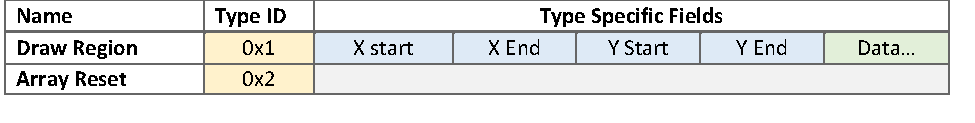
\includegraphics[width=1.0\textwidth]{fig/packet_chart.pdf}
    \caption{List of PDP Packets}
    \label{fig:packets}
\end{figure}

Figure \ref{fig:packets} shows the basic packets used for communication within PDP. These are strictly for data transfer and synchronization of system operations, and do not include other aspects such as system setup or enumeration\footnote{System setup and enumeration are typically system specific operations and outside of the current PDP Design, but may be incorporated in the future}. These packets are organized into type specific fields of some set word-size. The exact size of word fields is left abstracted to allow for an optimal implementation to be utilized in practice. For example, a system may utilize 24-bit word size if an array has a native 24-bit pixel size, or 32-bit word size if the hardware transport layer has a specific optimal word size. Typically, a multiple of 8-bit word size would be utilized in practice, as most hardware architectures (such as x86) utilize some multiple of this size. In any given implementation, the word size of all fields must match, in order to simplify decoding operations. This allows for fixed-size decoding of incoming data, which simplifies processing and firmware implementation; as well as, can ease timing constraints and enforce non-variability in the decoding time of incoming packets of data. In general, PDP packets are designed to send a minimal amount of header data to lower overhead and ordered in a way to minimize buffering requirements to enable real-time processing.

In terms of the protocol itself, PDP uses a single global coordinate system to refer to pixel locations on a display array. For example, a 512 by 512 pixel array would have coordinates from 0 to 511 in both the horizontal and vertical directions. All packets referencing sub-regions of this display would utilize coordinates that map to some rectangular sub-region of the display. Any overlapping regions of data would be composited during system operation with priority given to data segments sent at higher frame-rates.

PDP Packets are segmented into three types, a draw region packet, array reset packet, and trigger packet. All packets consist of a Type ID field of word-size. The draw region packet is used to send a rectangular sub-region of pixel data in global array coordinates. It has fields for the start and stop horizontal and vertical coordinates (defined inclusively) followed by individual pixel data. For example, suppose a scene generator were to send a packet of data from array region 10 to 19 along the X axis and 20 to 29 along the Y axis, a total of 100 pixels of data would follow the packet coordinates given that the packet specifies a 100 pixel sized region.

The second packet, array reset, is utilized to indicate that quadrants on a given array should be cleared. It consists of an array specific quadrant bit-mask used to indicate which quadrant to reset. Any unused bits are reserved. This type of packet would be utilized exclusively between compositor and array tile links.

The third packet, trigger, is used to implement a trigger based synchronization within in PDP. It consists of a system specific action bit-mask used to indicate the type of operation to trigger. In IRLED array systems, the coordinator of synchronization is dependent on the array itself and the different components within the system. In some systems, a sensor may be used as the source of synchronization, in other systems, another component may be utilized. Other aspects of system operation may even be triggered outside of the system synchronization interval based off of other events. For the reason, PDP has opted for a trigger based approach to synchronization. This approach allows for synchronization, data transfer, and computation to be custom tailored to an individual systems use-case. For example, the action mask could be used to trigger the generation of the next frame to be displayed when needed, the source of which is defined by the system itself. Another example would be utilize the action mask to indicate that further computations (such as scene generation) stall until otherwise indicated.

    \chapter{Machine Model}
        \label{chap:machine_model}

In this section, we will describe the abstract architecture upon which our PDP protocol operates in order to motivate the current and future use-cases for our protocol. Additionally, we will discuss how different components operate in the system in order to give the reader an intuition of the underlying operation.

\begin{figure}
    \centering
        \centering
        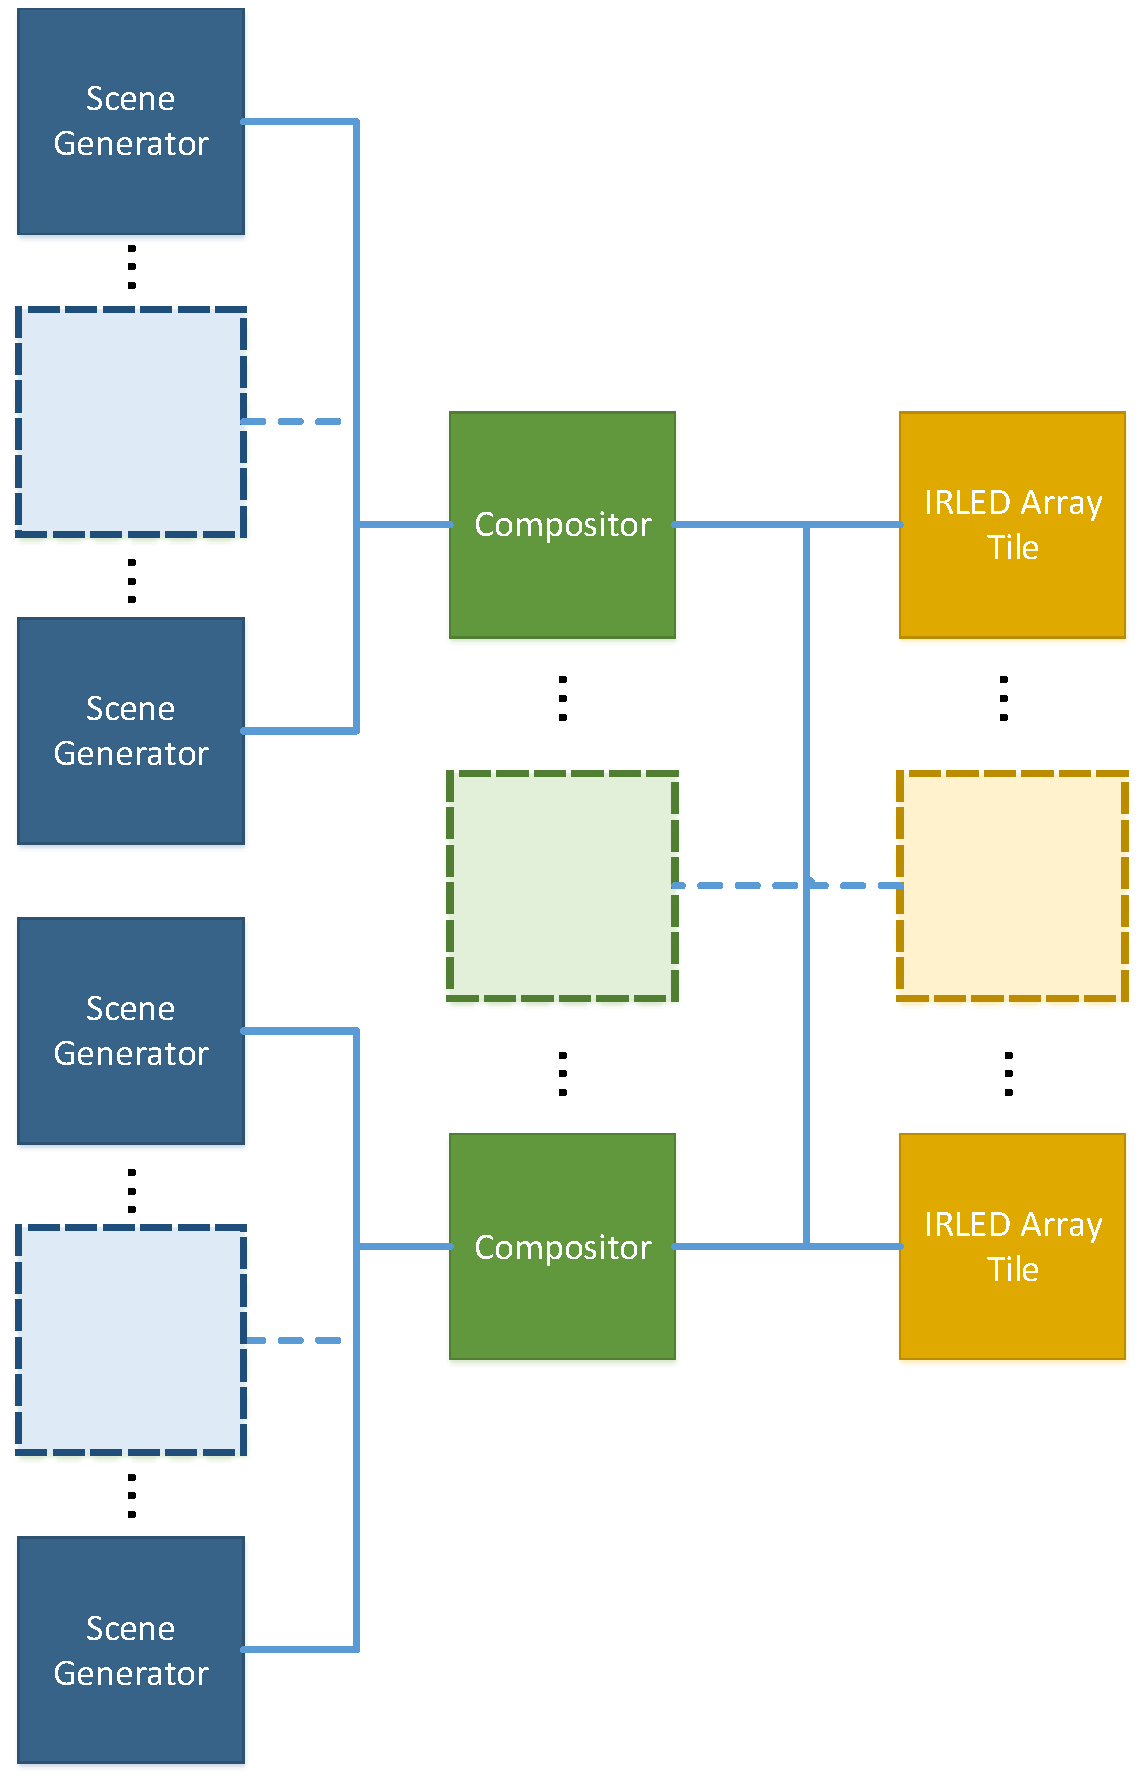
\includegraphics[width=0.75\textwidth]{fig/amm.pdf}
        \caption{Abstract Machine Model of our PDP architecture with 1-to-N relationships between components}
        \label{fig:amm}
\end{figure}

\begin{figure}
        \centering
        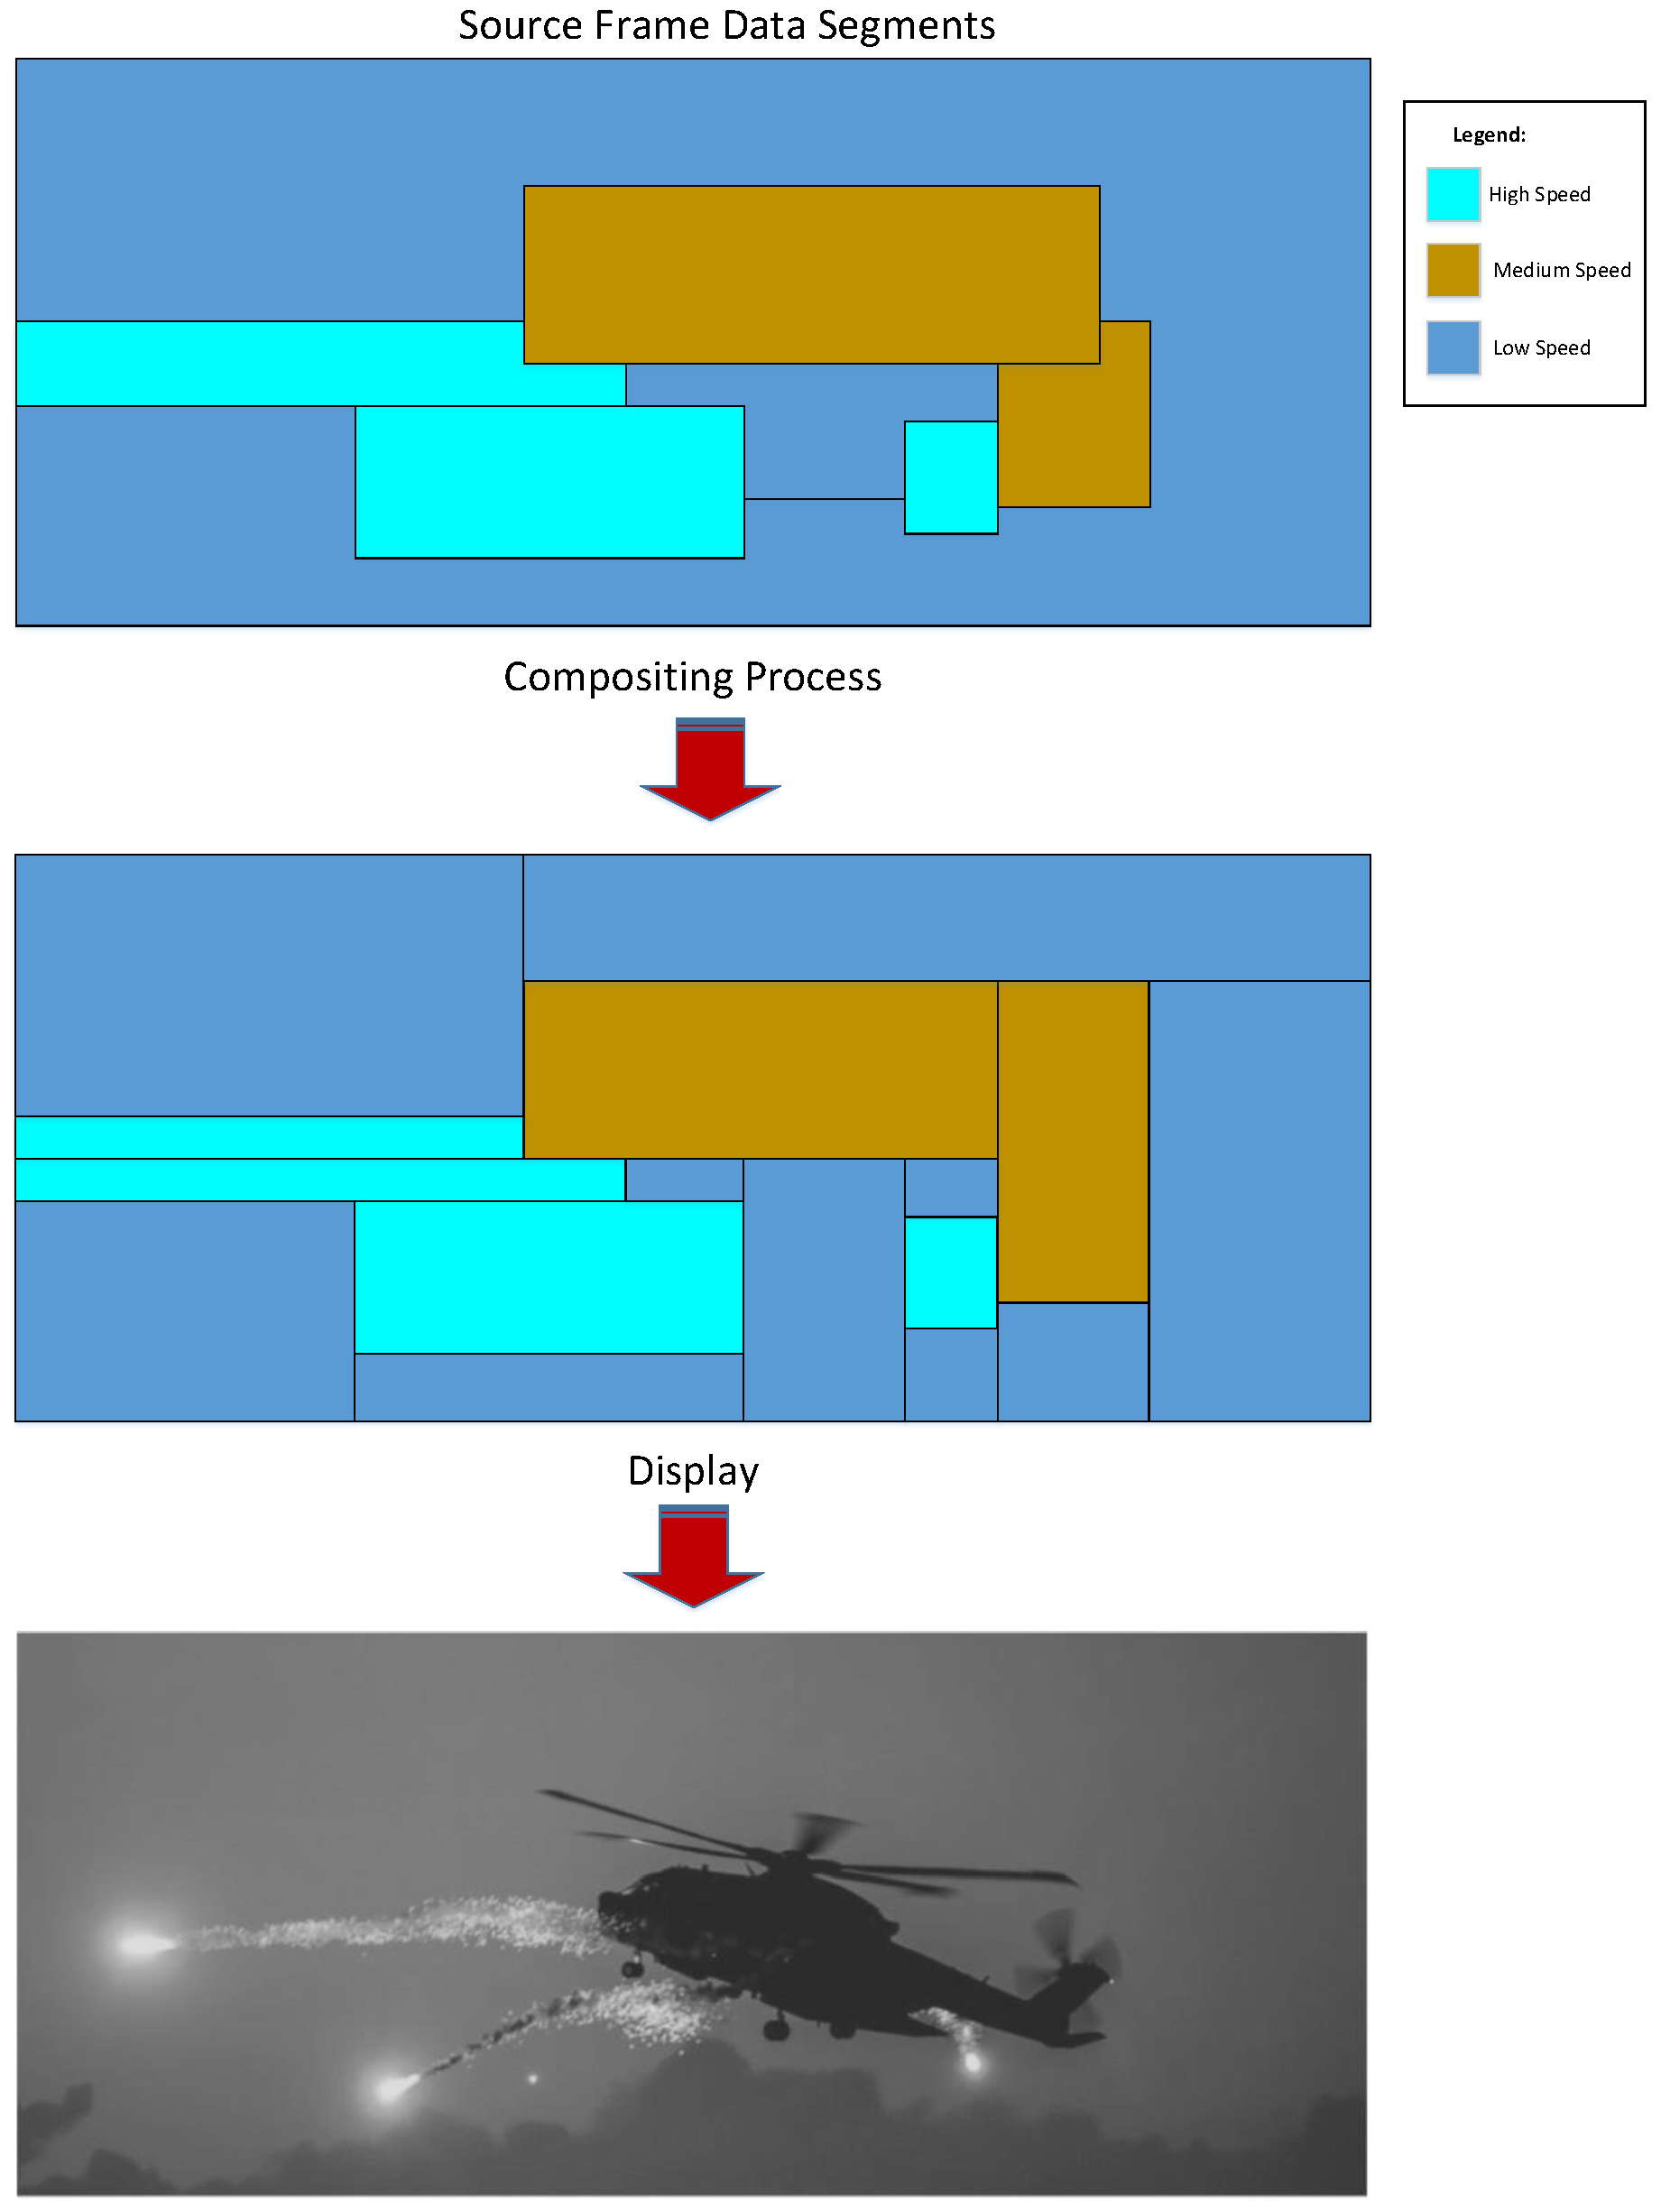
\includegraphics[width=0.85\textwidth]{fig/compositing.pdf}
        \caption{Compositing Process Example}
        \label{fig:compositing}
    \caption{Abstract Machine Model and Compositing Process}
\end{figure}


Traditional IRLED display systems are typically composed of three components as part of the display: scene generation, non-uniformity correction, and the actual display of InfraRed with sensors used to capture data. We propose an Abstract Machine Model (AMM) to capture these three components as shown in figure \ref{fig:amm}. This AMM separates the system operation of an IRLED system into three main components as well: scene generation, compositing, and display on IRLED array tiles with links between each component. The relationship between these components remains abstracted in such a way that hardware components may be scaled to fit demand. At its most basic, a single scene generator, compositor, and IRLED array tile may be used. For higher speed requirements, hardware components may be mapped as needed. The links between components in the system utilize the PDP protocol for communication, data-transfer, and synchronization. The compositing component differs from a traditional IRLED system in that it is responsible for taking imagery from many sources, possibly at different frame rates, and combining them into a single image for transmission to IRLED array tiles. This process is briefly shown in figure \ref{fig:compositing}. During the compositing process frame segments are ranked to determine which to send at high speeds, and which to send at low speeds for intelligent bandwidth utilization. Once segmented and ranked into non-overlapping speed classes, frame segments are transmits at the necessary rate.

For example consider the simple case, that of a single scene generator. In this case, the compositor will receive data from a single source. As frame data is received, a differencing algorithm must be employed to determine how to segment the overall frame for optimal data transfer based off of the rate of change of individual portions of the frame relative to the prior frame. Portions that rapidly change will be sent more often than portions that change slowly in order to maximize bandwidth for high-speed transfer of {\it hot} portions of an image. This consequently also has the effect of improving the performance of the analog chain of display devices by allowing for devices to reserve more time to drive rapidly changing portions of a display over portions of the display changing relatively slowly.

    \chapter{Use Cases}
        In this section, we provide an example scenario of the communication protocol in action within a simplified abstracted architecture. For demonstration purposes, the underlying details of the hardware are omitted and only the utilization of the protocol itself is examined.

Figure \ref{fig:frames} shows a series of frames segmented within PDP. For the purposes of this example, assume a system utilizing a single scene generator, compositor, and IRLED array. Assume also the average intensity of each region of a frame is computed during operation. The highlighted segments indicate a large change in intensity occurring within the region from frame to frame. Suppose that frames are generated at 4 times the rate of an external synchronization pulse. During operation within PDP, segments with a large change in intensity require higher frame-rate to reflect the fast frequency changes in intensity. The PDP protocol would be utilized to send these regions at a much higher frame rate than the slowly changing segments. Each segment would be sent using a region packet, one after another. Once sent, remaining time would be utilized by a compositor to send the slower changing data at a much slower rate. In this particular example, we could send the fast data for the frames at a rate much higher than that of the slowly changing segments; only updating the other segments once the fast moving data in all frames is sent. Once all data is sent, an external synchronization pulse from a sensor would then be utilized to indicate the data has been captured and a corresponding trigger packet sent from the compositor to scene generator to indicate that more frames be generated. The same procedure would then continue for the next set of frames.

\begin{figure}
    \centering
        \centering
        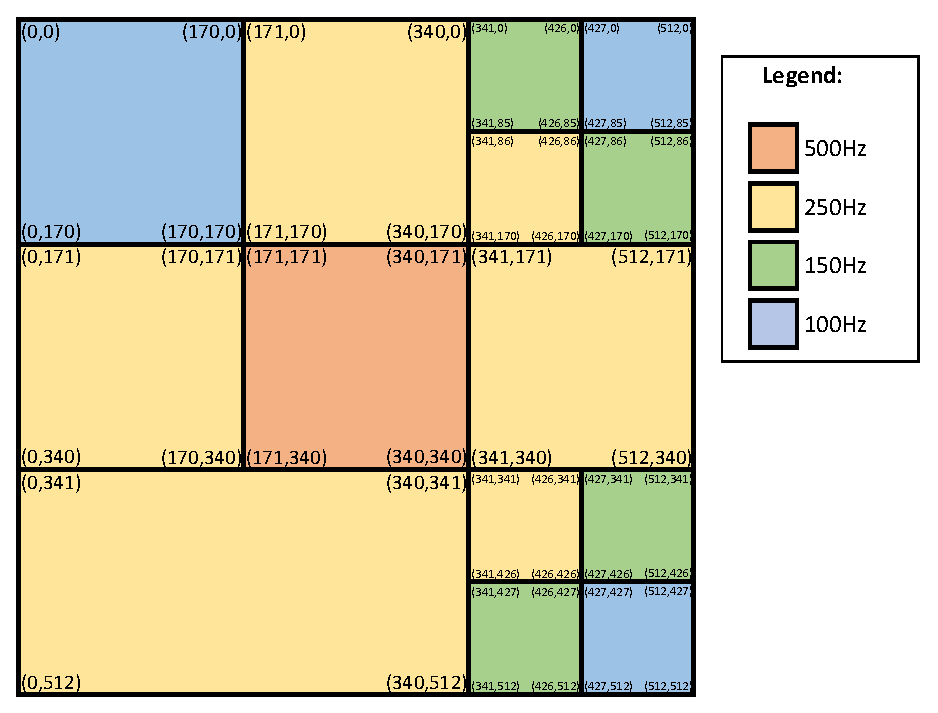
\includegraphics[width=1.0\textwidth]{fig/variable_display.pdf}
        \caption{Dynamic frame rate display with multiple regions updating at different frame rates}
        \label{fig:variable_display}
\end{figure}

\begin{figure}
        \centering
        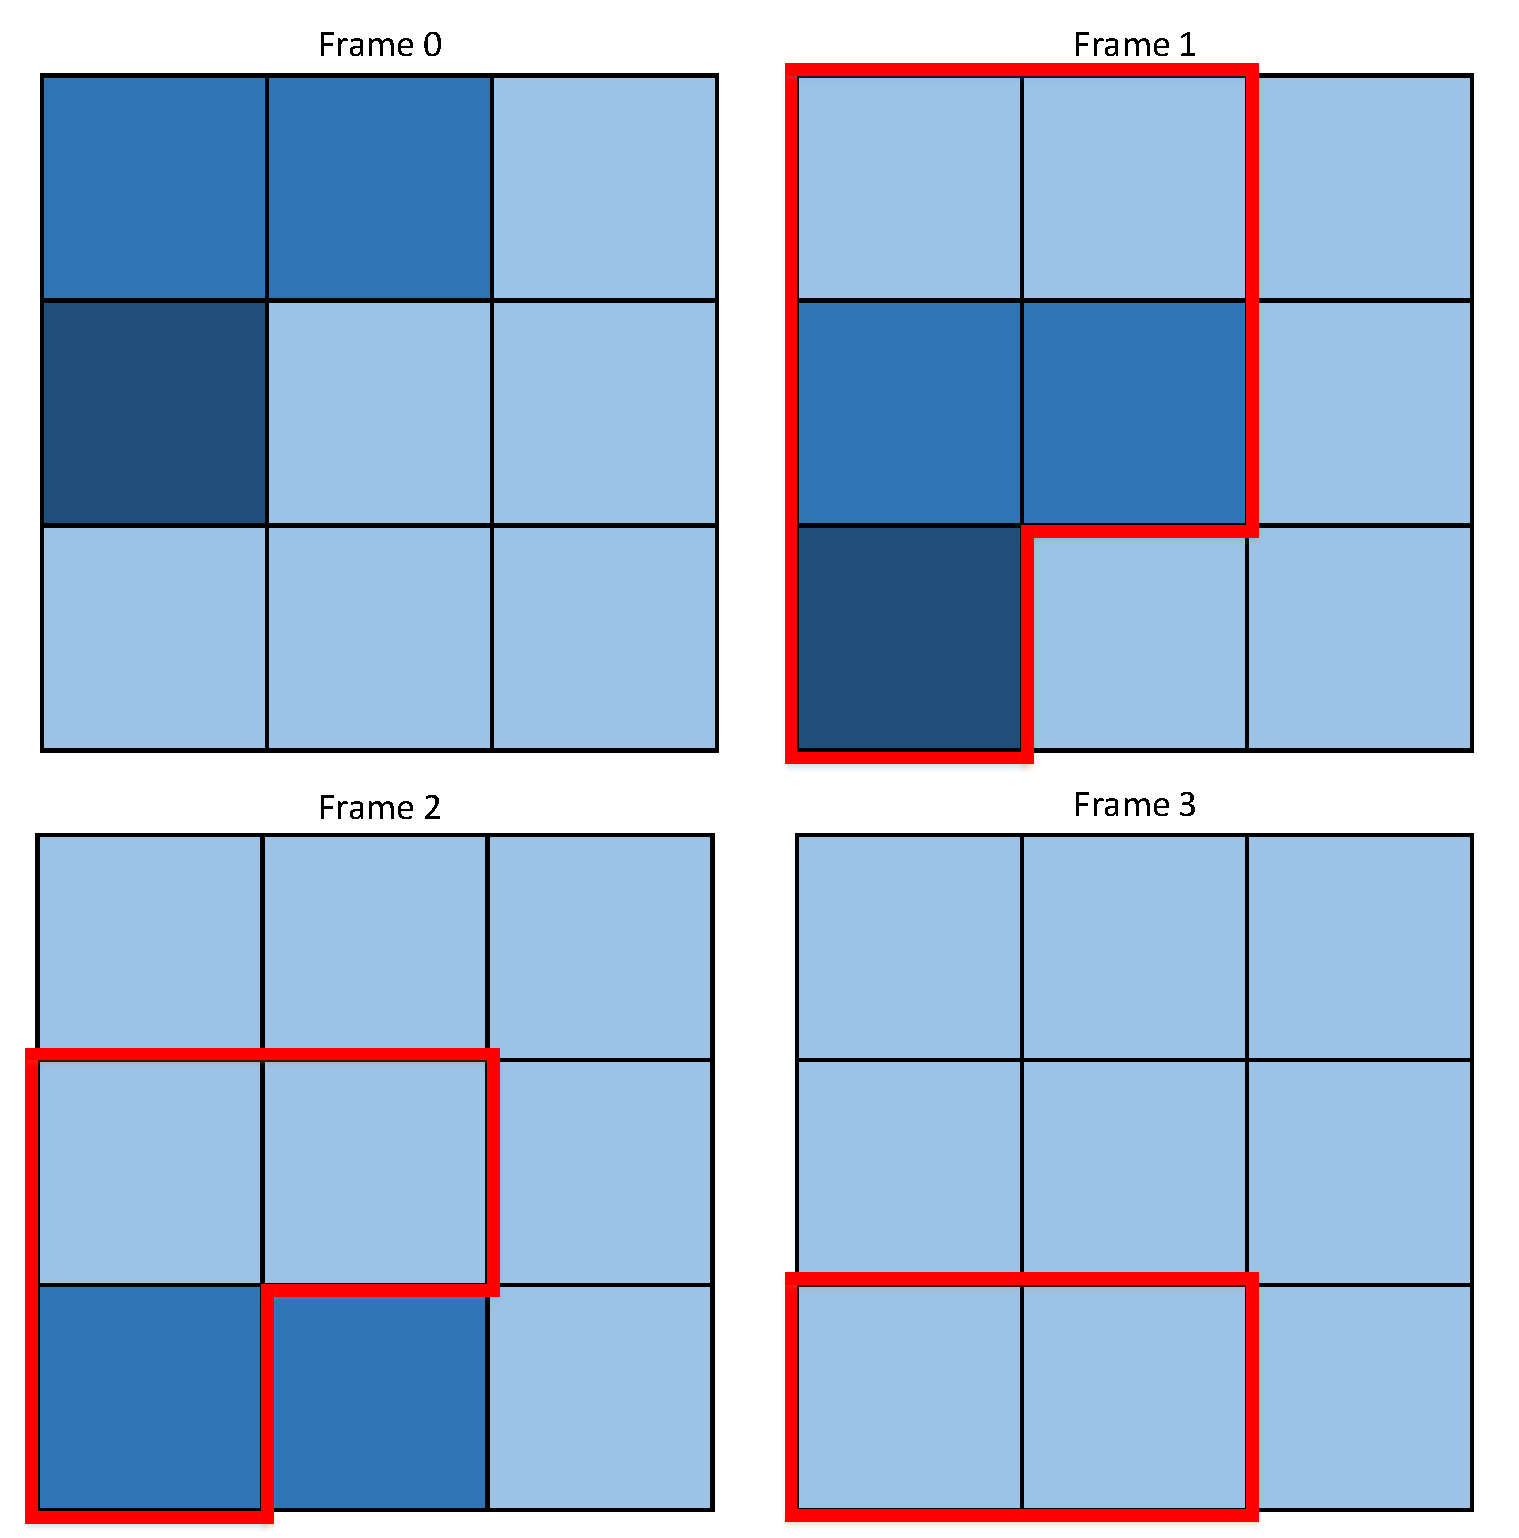
\includegraphics[width=1.0\textwidth]{fig/frames.pdf}
        \caption{Example display of frames within PDP. Each box indicates an average intensity for the given region}
        \label{fig:frames}
\end{figure}

In a real system, frames would be segmented more finely than in this example, allowing for small segments to be dynamically transmitted when needed. This would then give the ability for fast changing data to update at rates far greater than a static fixed frame rate display would be capable of doing under the same hardware considerations with limited bandwidth. Secondly, as discussed briefly above, this would give the analog portions of a display more time to settle thereby improving display fidelity. In more detail, the analog portions of a display are time constrained by the number of pixels that need to be addressed in a given time in fixed frame rate systems. By de-prioritizing slow changing data, these segments no longer need to be addressed at the same rate as the higher changing data in the display, allowing for more time for the high frame rate pixels to settle if needed.

    \chapter{Implementation}
        \label{chap:implementation}
%FIXME: my research group's arrays?
This chapter describes the implemented FPGA version of the PDP architecture used on my research group's arrays. For the purposes of this discussion, only relevant details are included to ease the readers understanding. First, the chapter will discuss the purpose of the implemented architecture. Following this each component will be discussed at a high level. Finally, the operation of sub-components will be discussed.

The implemented architecture consists of the portion of the AMM that drives an IRLED tile (or emitter array) directly from data packets sent by a compositor. As such, it is responsible for receiving PDP packets, decoding and validating them, and drawing them to an IRLED array. This is shown in Figure~\ref{fig:overall_arch}. In the current implementation, packets are sent using an underlying HDMI protocol layer. The incoming data is synchronized across two distinct clock domains utilizing a synchronized circular buffer (SCB). The input side consists of two separate HDMI inputs in order to meet system bandwidth requirements. Each input is assumed to contain clock skew relative to the other so separate SCBs are used to synchronize these to the system domain. At a high level, individual data words of 24-bit sized values come in per HDMI cycle. These are transitioned to the system domain and stored for retrieval by the array emitter module. The array emitter module is responsible for bringing in each 24-bit word value and emptying the corresponding SCB slot. As it brings in each word, it begins to decode them into PDP commands. Once enough data is buffered for a write or reset command, it sends the data to the write buffer module which then drives an emitter directly through IO lines.

%\begin{figure}
    %\centering
    \begin{figure}%{0.50\textwidth}
        \centering
        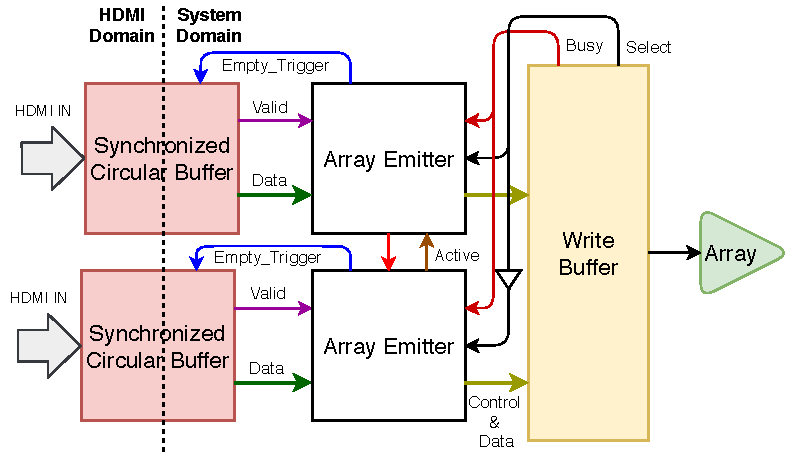
\includegraphics[width=1.0\textwidth]{fig/pdp_overall_arch.pdf}
        \caption{Overall PDP Architecture}
        \label{fig:overall_arch}
    \end{figure}%
    %\hfill
    \begin{figure}%{0.50\textwidth}
        \centering
        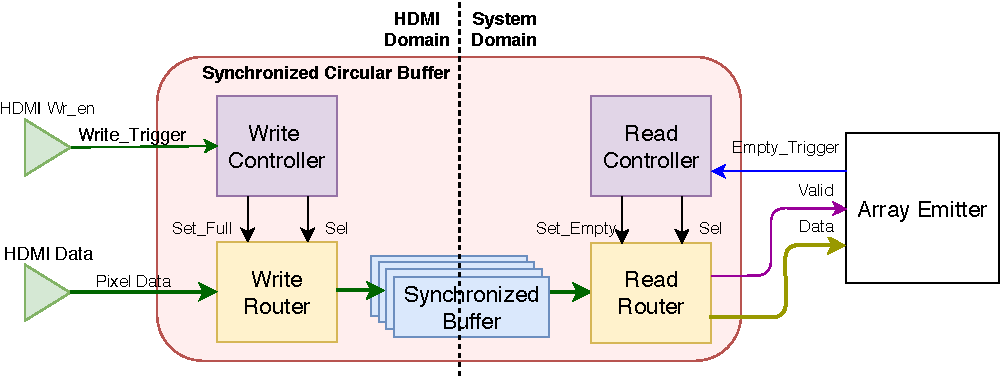
\includegraphics[width=1.0\textwidth]{fig/pdp_scb_arch.pdf}
        \caption{Synchronized Circular Buffer Architecture}
        \label{fig:scb_arch}
    \end{figure}
    %\caption{Overall Architecture \& SCB}
%\end{figure}

Figure~\ref{fig:scb_arch} shows the details of the synchronized circular buffer utilized in the implementation. Internally, it consists of two controllers, two data routers, and the actual internal buffer storage itself. The write controller is used to coordinate which internal buffer to write data to. A buffer is marked as full when a trigger comes in, and a new buffer is selected when the previous is filled. This is triggered via an external write enable signal sent from HDMI. The write router does the actual data redirection based off of the buffer selected by the write controller. Internally, a request-acknowledgment handshake is used to ensure the data has transitioned correctly across clock domains and is available on the other side. Once data becomes available, the read router will output the data lines, as well as, a valid signal indicating that the data can be read and cleared. The read controller will clear it once an empty trigger is sent from the array emitter indicating that the corresponding word has been read. It will then select the next buffer. Once the last buffer is written or read by either controller, the first buffer will be selected again. To note here for clarity, the actual filling and clearing of the buffers is done by HDMI write enable on the writer side, and the array emitter on the reader side.

Figure~\ref{fig:ae_arch} shows the details of the array emitter module used in the implementation. Internally, the array emitter consists of individual controllers that each perform a particular role. Currently these are the write enable controller, which controls writing draw region packets; the reset controller, which controls the resetting process per frame; and the valid controller which does validation checks on the input in order to verify the correctness of packets. Each controller takes in similar input signals and produces similar output signals with some exceptions depending on the actual function of the individual controller module. On the input side, each controller takes in a valid and data line corresponding to an individual word of a PDP packet. Additionally, an active line is brought into each controller to indicate whether another controller module is active or not. This is used to ensure that other modules do not become active (for correctness purposes) while another is currently processing a packet. During an idle phase, the write enable and reset controllers will wait for a corresponding packet ID to come in.

 \begin{figure}
    \centering
    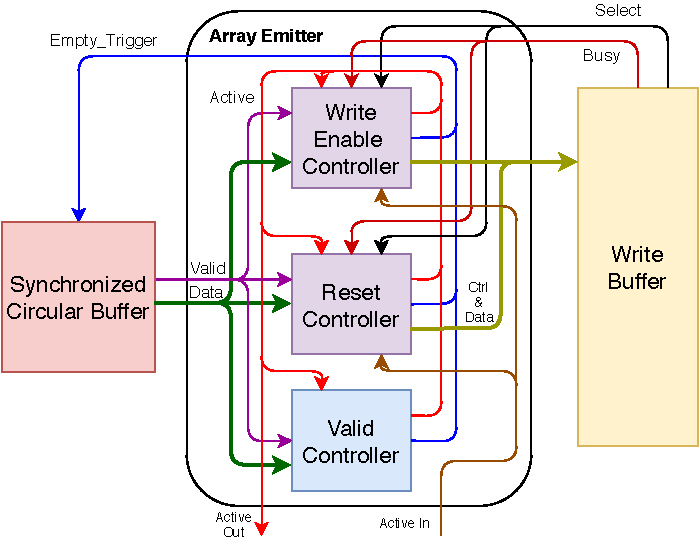
\includegraphics[width=1.0\textwidth]{fig/pdp_ae_arch.pdf}
    \caption{Array Emitter Architecture}
    \label{fig:ae_arch}
\end{figure}

When a packet ID matching an operation handled by a given controller arrives, the corresponding controller will switch states and then wait for the rest of the incoming packet data to arrive. This is shown in Figure~\ref{fig:state_machine}. For example, item 3 shows each state machine waiting for a corresponding PDP OP code. If a draw region packet ID were to arrive, then the state machine would wait for the X start address, X end address, Y start address, and Y end address shown in item 4. Finally, the state machine would buffer the needed data for a write and move to the write state once all data has been buffered. In the write state it would send the data to the write buffer. If more data needed to be written for the PDP packet, it would then continue buffering the needed data, and wait for the write buffer to be idle to send the next set of data. The busy line in Figure~\ref{fig:ae_arch} indicates when the write buffer is in the process of writing to the array. This would continue until all data was written for the packet, finally proceeding to the idle state. The reset controller contains similar logic, but for the reset process. The valid controller is used to ensure that incorrect or corrupt packet data is cleared. If an invalid packet OP code arrives during an array emitter idle phase, the valid controller will simply empty the corresponding SCB slot. In future revisions, it will perform CRC checks on packet data to ensure the header and body are valid. The Active-Out, Active-In, and Select lines are used to coordinate which array emitter module has control over the write buffer. After an array write, normally an array emitter will signal the write buffer that it is ceding control to the other array emitter, but only in cases where the other array emitter is currently active and waiting to write.

\begin{figure}
    \centering
    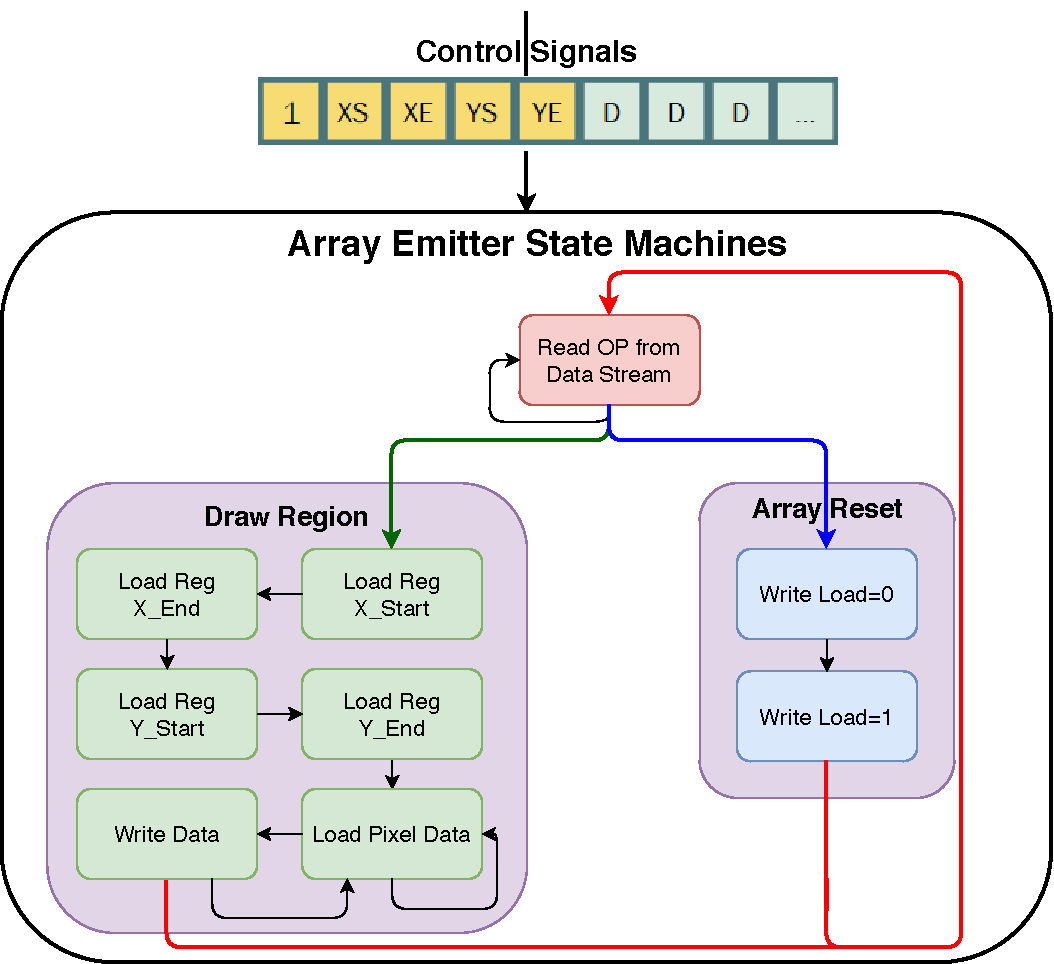
\includegraphics[width=1.0\textwidth]{fig/pdp_state_machine.pdf}
    \caption{PDP State Machine}
    \label{fig:state_machine}
\end{figure}

\section{Experimental Results}
This section provides a few captures of simulation inputs and outputs in order to show how packets arrive and are processed by the architecture.

In Figure~\ref{fig:input_example} simulated HDMI is shown. When video data enable (write enable) goes high words of data representing PDP packets start to stream in. These are indicated by Packet ID, X start, X end, Y start, Y end, and Packet Data. Each word would be stored in an SCB slot as indicated in the previous section. The final piece of data indicated is a reset packet. Note, that the data prior to Packet ID would be ignored as it does not represent a valid PDP command. It would be discarded by the valid controller.

\begin{figure}
    \centering
    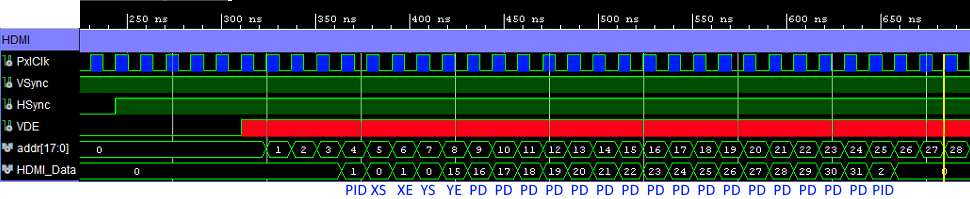
\includegraphics[width=1.0\textwidth]{fig/pdp_input_example.png}
    \caption{PDP Single HDMI Input Example Simulation}
    \label{fig:input_example}
\end{figure}

Figure~\ref{fig:output_example} shows the final output driven to the array. Highlighted in red is data from the write enable packet. Note, all values out are up shifted by 5 bits to be received by the DACs in the system. Additionally, the values are shown in reverse order from the input diagram. For example, 992 corresponds to the value of 31 on the input side. In purple the reset packet is shown with two stages of array writes. In the first stage, load line goes low. In the second stage the load line goes high.

\begin{figure}
    \centering
    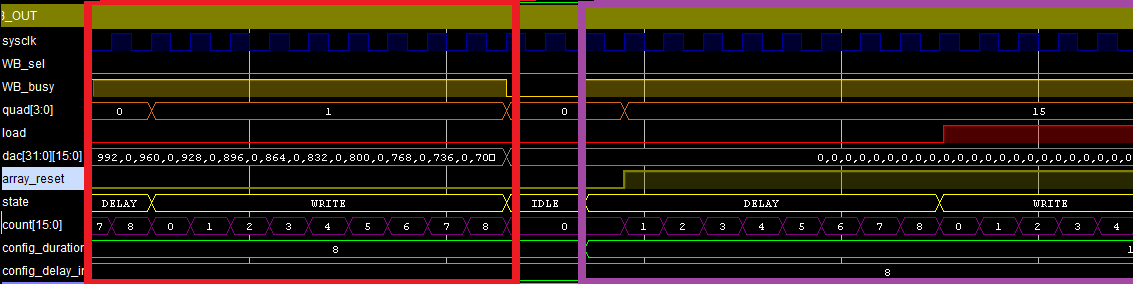
\includegraphics[width=1.0\textwidth]{fig/pdp_output_example.png}
    \caption{PDP Output Example Simulation}
    \label{fig:output_example}
\end{figure}

    %\chapter{Simulation Framework}
        %\input{Text/Framework}
    %\chapter{Experimental Evaluation}
        %This section provides a few captures of simulation inputs and outputs in order to show how packets arrive and are processed by the architecture.

In Figure~\ref{fig:input_example} simulated HDMI is shown. When video data enable (write enable) goes high words of data representing PDP packets start to stream in. These are indicated by Packet ID, X start, X end, Y start, Y end, and Packet Data. Each word would be stored in an SCB slot as indicated in the previous section. The final piece of data indicated is a reset packet. Note, that the data prior to Packet ID would be ignored as it does not represent a valid PDP command. It would be discarded by the valid controller.

\begin{figure}
    \centering
    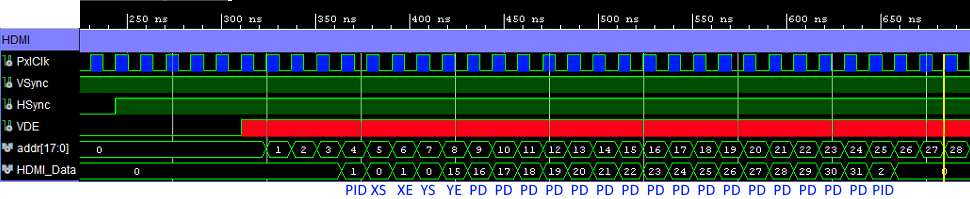
\includegraphics[width=1.0\textwidth]{fig/pdp_input_example.png}
    \caption{PDP Single HDMI Input Example Simulation}
    \label{fig:input_example}
\end{figure}

Figure~\ref{fig:output_example} shows the final output driven to the array. Highlighted in red is data from the write enable packet. Note, all values out are up shifted by 5 bits to be received by the DACs in the system. Additionally, the values are shown in reverse order from the input diagram. For example, 992 corresponds to the value of 31 on the input side. In purple the reset packet is shown with two stages of array writes. In the first stage, load line goes low. In the second stage the load line goes high.

\begin{figure}
    \centering
    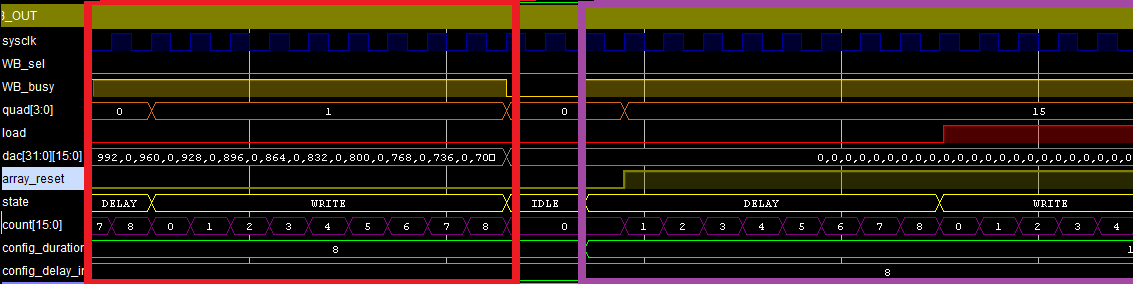
\includegraphics[width=1.0\textwidth]{fig/pdp_output_example.png}
    \caption{PDP Output Example Simulation}
    \label{fig:output_example}
\end{figure}

    \chapter{Related Work}
        \label{chap:related_work}

    \chapter*{Conclusion}
    \addcontentsline{toc}{chapter}{conclusion}
        \label{chap:conclusion}
In this paper, we described a packetized display protocol architecture and associated abstract machine model to convey the limitations in current fixed frame technology. Additionally, we provide an alternative display architecture that eschews the design decisions of current technology in order to provide intelligent dynamic bandwidth utilization, fine-grained control over frame transmission and synchronization; as well as, allows for dynamically changing intra-frame rates. We believe this architecture has the potential to provide the capabilities to bridge the performance gap found in current technology, and will serve as a better-fit solution for future high performance IRLED systems due to the scalable nature of the design and the carefully incorporated abstraction tailored to allow for different types of hardware and system setups to utilize the PDP architecture. Care has been taken in the design to incorporate many different possible system setups without limiting the use-case of PDP to a specific hardware setup; while at the same time, considering firmware implementation and timing aspects to packet decoding.

Current work includes a FPGA based implementation of a PDP decoder architecture utilizing HDMI. We have provided both a description of the implemented architecture, as well as, simulated sample data running on the architecture. Future work includes testing the architecture on an emitter array, performing scalability testing, and comparing the results to a classic architecture at matching pixel clock rates in order to show effective speedup with varying packet sizes. Further work is to be done to demonstrate dynamic frame-rates in action on an array. Finally, a CRC is to be implemented to ensure correct operation at all times. We also wish to scale the number of inputs in order to increase the effective hardware bandwidth further than capable with a classical system.


    %FIXME: Ack and Disclaimer
    \section*{Acknowledgment}
        The work discussed within this dissertation was partially funded by (a) Air Force STTR Program AF18A-T017 `Next Generation Infrared Scene Projectors for Testing MWIR Systems' (Contract FA8650-19-C-1948), and (b) the Test Resource Management Center (TRMC) Test and Evaluation/Science \& Technology (T\&E/S\&T) Program through the US Army Program Executive Office for Simulation, Training, and Instrumentation (PEO STRI) under Contract No. W900KK-13-C-0049. I thank ONSemiconductor from fabricating silicon arrays, Firefly Photonics and the University of Iowa for fabricating Infrared LED arrays and Teledyne Scientific for hybridizing Silicon and LED arrays. Their fabrication effort enabled us to build and test the projector system(s) described in this paper.

    \section*{Disclaimer}
        This report was prepared as an account of work sponsored by an agency of the United States Government. Neither the United States Government nor any agency thereof, nor any of their employees, makes any warranty, express or implied, or assumes any legal liability or responsibility for the accuracy, completeness, or usefulness of any information, apparatus, product, or process disclosed, or represents that its use would not infringe privately owned rights. Reference herein to any specific commercial product, process, or service by trade name, trademark, manufacturer, or otherwise does not necessarily constitute or imply its endorsement, recommendation, or favoring by the United States Government or any agency thereof. The views and opinions of authors expressed herein do not necessarily state or reflect those of the United States Government or any agency thereof.

    \renewcommand{\bibname}{References}
    \pdfstringdefDisableCommands{\let\uppercase\relax}
    \bibliography{Bib/biblio}
    \bibliographystyle{ieeetr}

\end{document}
